\chapter{Models of Process}

Integrative systems modeling (ISM) combines system dynamics modeling with statistical modeling, by using a ``mechanistic'' model of process together with a statistical model of data.  The foundations of ISM are best articulated in terms of \emph{system dynamics modeling}, a discipline that originated in the fields of operations research and industrial engineering \cite{TK original works on GM, city, globe, systems thinking primer}.  This type of compartmental modeling is similar to infectious disease modeling \cite{andersen and may, rohit and premanji, vcycychy and, diekman and other} and pharmacokinetic modeling \cite{jacquez1, jacquez2}.

System dynamics modeling is a method to model the behavior of complex systems in terms of stocks, flows, and feedback loops.  In short, \emph{stock variables} quantify the amount of some material, or mass, or population in a compartment at a particular moment in time, while \emph{flow variables} quantify the rate of material moving into, out of, or between compartments. The scope of applications for system dynamics is enormous, and once you start thinking of systems in this way, it may seem that everything can be modeled as stocks and flows. This method has been applied to the study of complex systems in economics, politics, environmental science, and a diverse array of other fields (see \cite{Meadows_Thinking_2008,Jacquez_Modeling_1999,Harte_Consider_1988} for an introduction to this modeling approach).

Traditionally, there is a delineation between system dynamics modeling and statistical modeling in the following way: system dynamics aims to develop a \emph{model of process}, while statistical approaches focus on developing a \emph{model of data}. Models of process attempt to explicitly represent the mechanisms behind some system behavior (deterministically or stochastically), while models of data often explicitly avoid requiring such a theory. The advantage of using the system dynamics approach is that it can incorporate structural assumptions about the system.  However, in many applications, the systems-dynamics model of process is not connected to data at all.  On the other hand, in many statistical approaches, the domain-specific dynamics of the system under study are not incorporated in the model explicitly, and the data models could benefit from this additional structure.  Integrative systems modeling is a framework to bring together a model of process and a model of data for mutual benefit.

\subsection{A simple example}

An example will help to make these concepts more concrete.  We begin with the simplest of compartmental models, a single compartment with in-flow and out-flow and no feedback, shown schematically in Figure~\ref{forward-sim-one-compartment}.

\begin{figure}[h]
\begin{center}
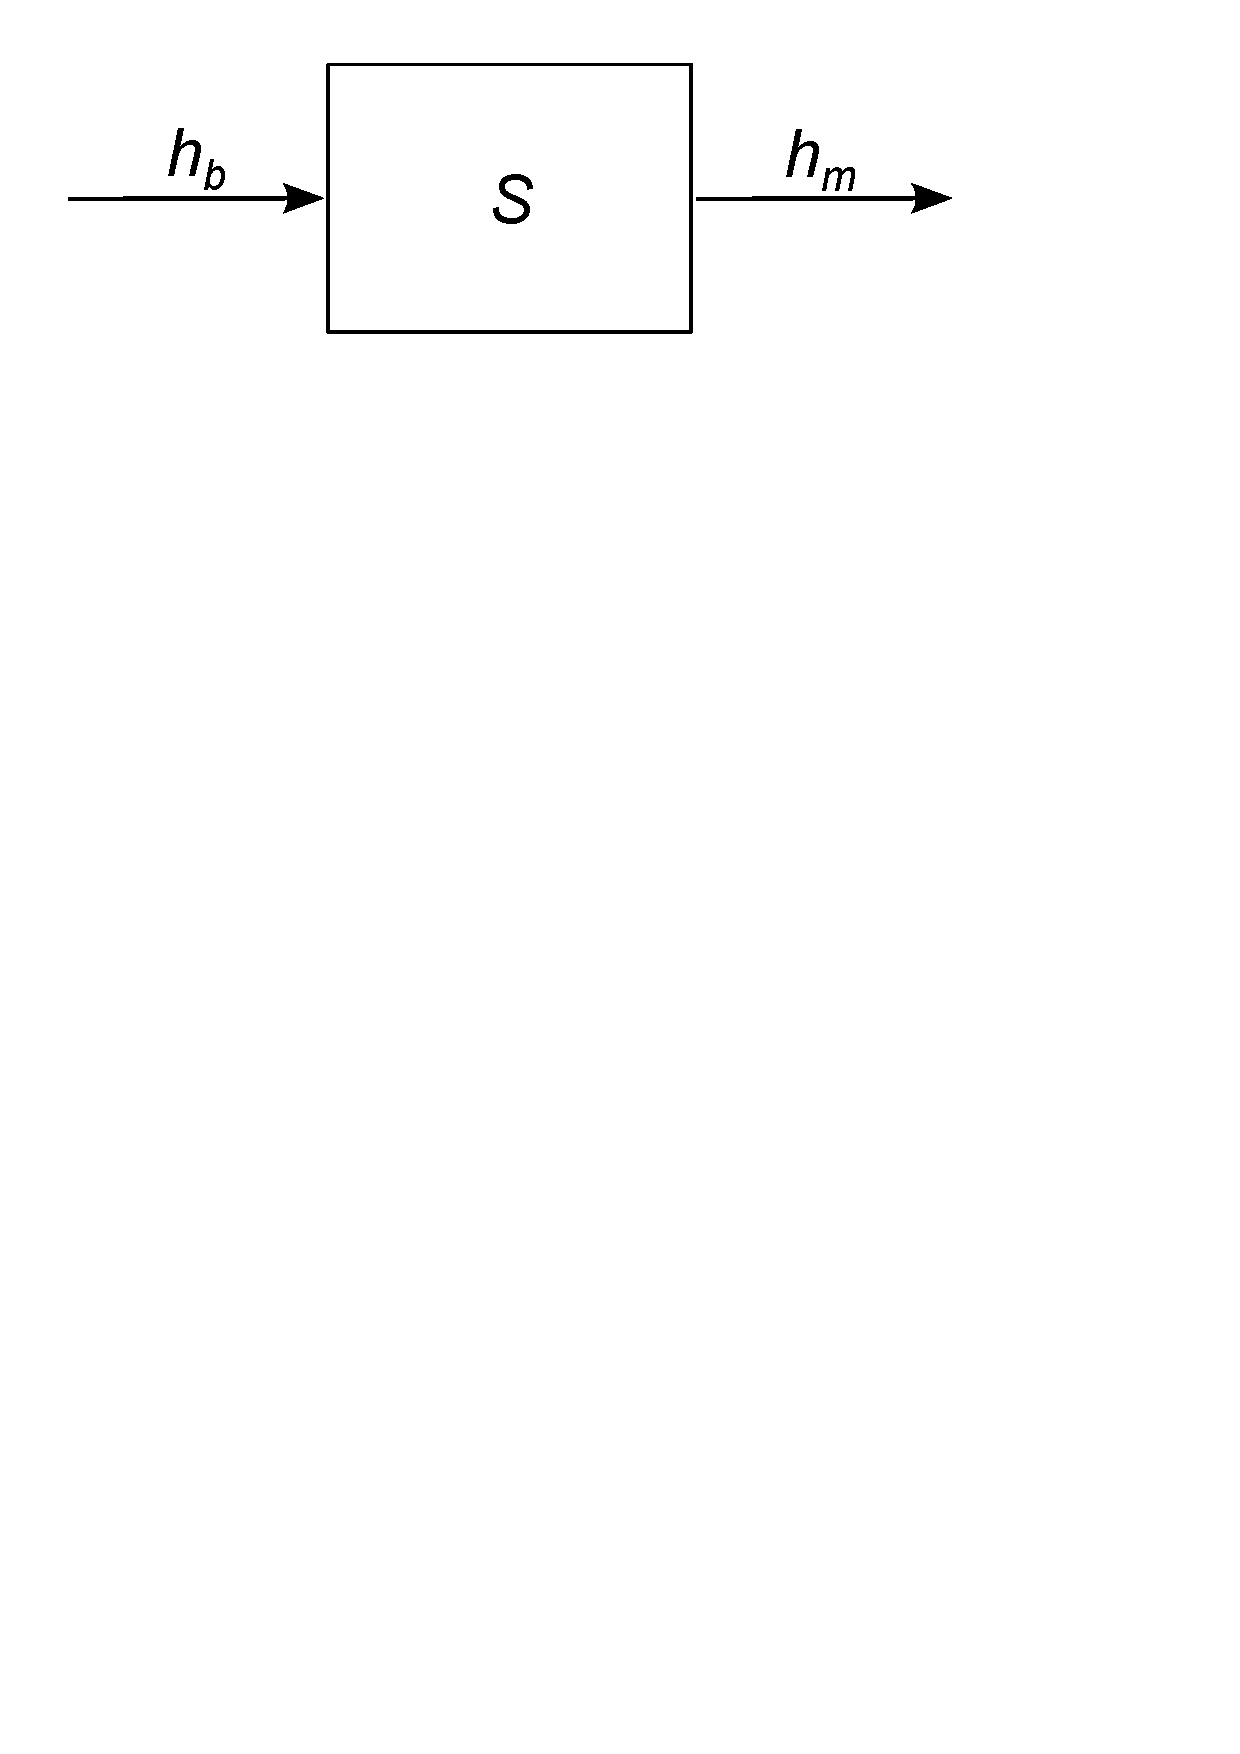
\includegraphics[width=3in]{S.pdf}
\caption{A single compartment model with in-flow $b$ and out-flow $m$ is one of the simplest examples of a compartmental model. Despite its simplicity, it is a useful model of population dynamics.  In this application, $b$ represents the birth rate, and $m$ represents the mortality rate, while $S$ represents the ``stock'' of population.}
\label{forward-sim-one-compartment}
\end{center}
\end{figure}


Schematic diagrams stock-and-flow models such as Figure~\ref{forward-sim-one-compartment} are useful in understanding and communicating the structure of a model of process, but they are incomplete. The full description is represented in the form of a system of difference equations or differential equations which specify precisely the relationship between the stocks and flows. The following differential equation fully specifies the one-compartment model:

\[
\frac{dS}{dt} = (b - m)S.
\]

In this equation, the stock $S$ changes continuously, increasing with birthrate $b$ and decreasing with mortality rate $m$. When $b$ and $m$ are constants, this differential equation has a closed-form solution, of $S = S_0 e^{(b-m)t}$. When $b$ and $m$ are not constant with respect to time, the model does not necessarily have a closed form solution, and many more time trends are possible for $S$.  Figure~\ref{forward-sim-one-compartment-soln} shows the time trend of $S$ when $b$ and $m$ are constant in panel (a) and when they are changing in panel (b).

\begin{figure}[h]
\begin{center}
\includegraphics[width=3in]{TK.pdf}
\caption{TK figure showing solution of one-compartmental model, with caption giving all of the details.}
\label{forward-sim-one-compartment-soln}
\end{center}
\end{figure}


\subsection{Related Work}

The field of system dynamics, from which ISM borrows terminology and inspiration, developed in management science. An early application was in explaining employment cycles at a large company's appliance plants \cite{Forrester_Counterintuitive_1971}. The prevailing theory of the time was that hiring and firing cycles followed general, economic cycles. However, a compartmental model of the system underlying the appliance business showed that the employment cycles arose from feedback loops inherent to company's internal structure, and could be smoothed out by modifying conditions entirely under the company's control. This first application demonstrates a major theme in system dynamics. In complex systems, determinants of system behavior considered one-by-one may be insufficient to predict the behavior of that system. The most important behavior in a complex system arises out of interactions and feedback between processes in that system---this is also the case in disease modeling where the dynamic nature of the disease process should be taken into account. The information contained in modeling the entire disease process---including incidence, remission and mortality---for a given disease, can exceed the information contained in separate analyses of that disease's mortality, incidence, and remission separately. There is increasing interest in applying system dynamics to solve a number of diverse health issues that require a model with sufficient complexity to incorporate multi-causal relationships. Fields such as pharmacology, epidemiology, and public health have applied compartmental models to tackle a range of interesting modeling challenges.

Pharmacokinetic and pharmacodynamic (PKPD) modeling, a subdiscipline of pharmacology, developed an approach to compartmental modeling in tandem with system dynamics modeling, largely independently.  However, the mathematics behind the models of process are extremely similar. The compartments in PKPD models represent organs and other physical systems in the body, and stocks represent the quantities of pharmacologically relevant compounds in these compartments.  The flows model the process of the drug of interest being metabolized or otherwise passing through the subject. Mathematically, these models have precise parallels to the stock-and-flow models developed 
for supply chain analysis. For instance, in one experiment researchers used a system dynamics approach to model glucose kinetics \cite{Gastaldelli_Glucose_1997}. They found that a three compartment model where two compartments correspond to peripheral pools exchanging plasma at different rates with a central pool best represented the physiology of glucose kinetics in their test subjects (in this case, a sample of 7 sheep). This particular model structure has arisen several times in applications in pharmacokinetics. It is called the mammillary model. In another experiment, researchers modeled the kinetics of epsilon-aminocaproic acid (EACA) in 6 human subjects. EACA is a compound used to control hemorrhage in patients with bleeding problems. The PKPD researchers developed a multi-compartmental model, where EACA was infused in a central compartment, distributed to fast and slow excreting peripheral compartments, and cleared by two compartments, one representing renal excretion of the drug, and another representing non-renal excretion \cite{Frederiksen_Kinetics_1984}.  In both of these examples, and in general practice in pharmacokinetics, the compartmental model of process is connected to a statistical model of data. This connection is the central idea of integrative systems modeling, and will be developed in detail in later chapters.

One area in which public health has a long tradition of compartmental and system dynamics modeling is in infectious disease \cite{Anderson_Infectious_1991, Hethcote_Qualitative_1976, Blower Hypercube sampling}. For example, the Susceptible-Infected-Recovered compartmental model, which was discussed in Section~\ref{TK}. This basic model has been extended in a variety of ways in order to model increasingly more complex infectious disease dynamics. For instance, in one study Nagelkerke and colleagues modeled the impact of a range of interventions targeted at preventing transmission of HIV/AIDS epidemics \cite{ref}. They estimated impact using a compartmental model where the population moved from an ``Uninfected'' compartment to either treated or untreated ``Infected'' compartments to an ``AIDS'' compartment to a ``Death from AIDS'' compartment. 

Another example that makes an explicit connection between epidemiological modeling and system dynamics is the recent work by Kershenobich and colleagues, who applied a systems approach to forecasting the prevalence of hepatitis C. They developed a compartmental model tracking incidence, diagnosis and treatment of the disease. For the incident population in the model, an individual moves from an acute phase (which lasts for 6 months) to a chronic phase, unless that individual is spontaneously cleared of the disease, is treated and cured or dies. For the prevalent population in the model, an individual moves from viraemic to non-viraemic, dies or gets treated and cured. Separate models were also used to estimate the mortality rate in different countries based on age, liver-related deaths due to hepatitis C infection, and percent of the population infected by injection drug users. Sensitivity analyses were conducted by running the model for a number of input scenarios.  TK description of what this model allowed the authors to do, and especially how hard it would have been to do in any other way.

Health systems are particularly complex, with many actors and many feedback loops, providing a large supply of systems modeling opportunities. The health of a population is affected by a combination of biological, economic, demographic, and political forces, and all of these spheres interact in a unexpected ways. Since the 1970s, system dynamics models have been applied to model these various forces in order to advance our understanding of population health \cite{refs TK[KP6][ADF7]]}. The topics addressed have included: disease epidemiology, substance abuse epidemiology, patient flows in emergency care, health care capacity and delivery, and interactions between health care and disease epidemiology. A systems approach is often required, because isolating one part of a public health problem and then addressing that may in fact adversely affect other parts of the system. For instance, low tar/nicotine cigarettes were developed to address one part of the burden of disease caused by tobacco consumption, but consumer behavior was not taken into account. Consumers tended to take longer, more frequent drags and thus negated the benefit of the low tar/nicotine content \cite{Sterman_Learning_2006,[ref [KP8]TK]}. A system approach would seek to simultaneously account for both the effect of the tobacco product on the consumer and the consumer's behavior. In the context of modeling the progression of a disease through a population, a model that seems to describe infection dynamics accurately may conflict with data on remission or fatality. Only by modeling the three together can the analyst get the most accurate and consistent estimates.

In another health system-focused example, Flaxman and colleagues developed a stock-and-flow model to synthesize data on the availability and distribution of insecticide treated bednets (ITNs) and to predict the proportion of households who owned an ITN. This analysis employed a Bayesian approach to estimate the parameters of the compartmental model that describe the process of ITNs moving from warehouses and other storage facilities into the household and possibly getting discarded by the households or lost in the distribution process.  This approach is commonly used by pharmaceutical firms to track their product.

These examples provide a basic understanding of the myriad uses for systems dynamics modeling. The following chapters will detail how these same ideas can be applied to a model-based meta-regression tool for disease modeling. 




TK connection to the references cited in this NIH RFP for systems modeling
\url{http://grants.nih.gov/grants/guide/pa-files/PAR-08-224.html}
\url{http://ajph.aphapublications.org/cgi/content/full/96/3/452}
\url{http://www.hpsig.com/images/f/f5/SD_background_for_public_health_%284.11.05%29.pdf}
\url{http://www.systemswiki.org/index.php?title=Health_System_Dynamics_References}
\url{http://www.chronicdisease.org/nacdd-initiatives/diabetes/professional-development/act-on-data/SDMResourceList.pdf}



TK transition paragraph going from ISM in general to the specific model to be used in model-based meta-regression for the GBD.

\section{System dynamics model of disease in a population}

The heart of the model-based meta-regression framework, to which this book is devoted, is a two-compartment system dynamics model of process, which represents the ``fundamental equations'' of population health. The compartments contain the population susceptible to the disease (stock $S$, for ``susceptible'') and the population with the condition (stock $C$, for ``condition''). The population moves between these compartments following the arrows shown in Figure~\ref{forward-sim-two-compartment}, transitioning from $S$ to $C$ with incidence rate $i$, and from $C$ back to $S$ with remission rate $r$. The susceptible population flows out of the system with (without-condition) mortality rate $m$, and the with-condition population flows out of the system with with-condition mortality rate $m+f$.  Here $f$ represents the ``excess mortality rate'' for individuals with the condition over individuals without the condition.

\begin{figure}[h]
\begin{center}
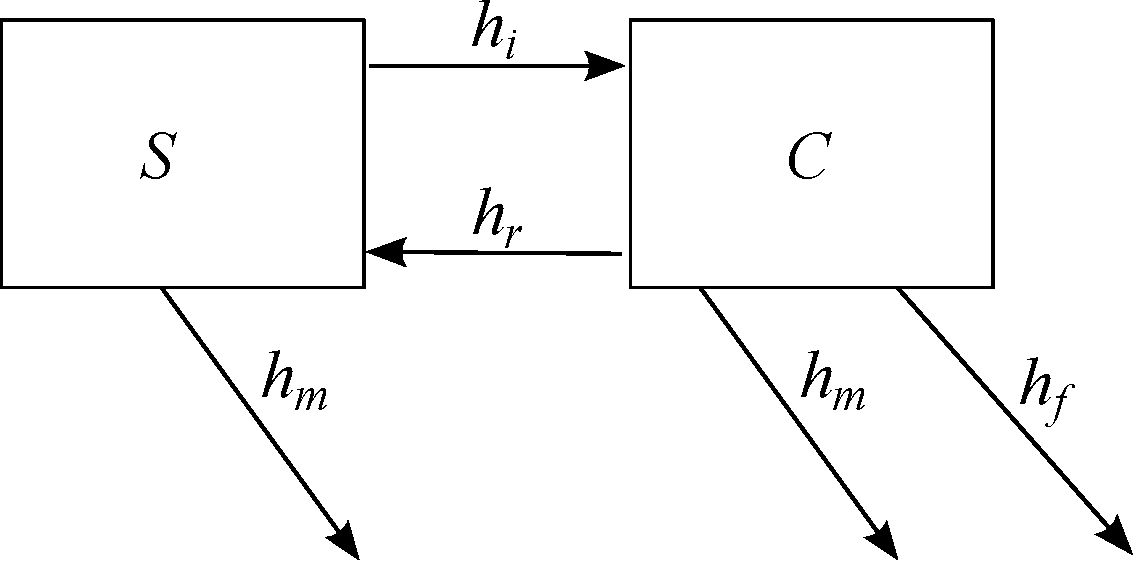
\includegraphics[width=5in]{SC.pdf}
\caption{The two-compartment model of process for disease in a population, around which the meta-regression framework is built. Compartment $S$ contains the population susceptible to the disease and compartment $C$ contains the population with the condition. Individuals move from $S$ to $C$ with incidence rate $i$, and from $C$ to $S$ with remission rate $r$. The susceptible population flows out of the system with without-condition mortality rate $m$, and the with-condition population flows out of the system with with-condition mortality rate $m+f$, where $f$ is the excess mortality rate, representing quantitatively the increase in mortality for individuals with the condition.}
\label{forward-sim-two-compartment}
\end{center}
\end{figure}


This ``model of process'' looks deceptively simple, and compared to the complex systems often developed in infectious disease modeling it \emph{is} quite simple.  However, it is no simpler than needed, and matches well the myriad of available data about the descriptive epidemiology of disease.  In the coming sections, we will connect this model of process to an appropriately complex model of data, and together they will provide our integrative systems model for model-based meta-regression.

There is an analogy of this simple model of process to the basic demographic equation of demography (also known as the fundamental balancing equation) \cite{TK book on demography}, which says that the population at time $t+\Delta t$ is equal to the population at time $t$, minus the number of deaths, plus the number of births, minus out migration, plus in migration:
\[P_{t+\Delta t} = P_t + B_{t, \Delta t} - D_{t, \Delta t} +
 I_{t, \Delta t} - E_{t, \Delta t},
\]
where $P_t$ is the population at time $t$, $B_{t, \Delta t}$ and $D_{t, \Delta t}$ are the number of births and deaths between time $t$ and $t+\Delta t$, and $I_{t, \Delta t}$ and $E_{t, \Delta t}$ are the number of immigrants and emigrants from the population between time $t$ and $t+\Delta t$.

As mentioned in the previous section, a schematic depiction of a compartmental model, such as Figure~\ref{forward-sim-two-compartment}, is not a complete description of the system dynamics.  To specify them completely I now turn to a system of partial differential equations, which correspond to the stocks and flows above, and more precisely represent their relationship as a function of time and age: 
\begin{align*}
\frac{\partial S}{\partial (a+t)} &= -(i + m)S + rC,\\
\frac{\partial C}{\partial (a+t)} &= iS - (r + m + f)C,\\
\end{align*}
where
\begin{align*}
S &= S(a,t) = \text{stock of ``susceptibles''},\\
C &= C(a,t) = \text{stock of ``with condition''},\\[.1in]
i &= i(a,t) = \text{incidence rate for susceptibles},\\
r &= r(a,t) = \text{remission rate for individuals with condition},\\
m &= m(a,t) = \text{without-condition mortality rate for any individuals},\\
f &= f(a,t) = \text{excess-mortality rate for individuals with
condition}.
\end{align*}
In general, all of these quantities are functions of both age $a$ and time $t$.

Although this section of the book is devoted to the model of process, and the model of data will be elaborated in great detail in subsequent sections, it is valuable to pause here and consider what descriptive epidemiological data may be collected in a systematic review of the literature and how it corresponds to the stocks and flows in the model.

For certain especially infectious diseases, cases identified in the health system are required to be promptly reported to the WHO; for example, the incidence of TB.  This yields data on disease incidence rates (which is not age-specific, i.e. crude incidence rate over all ages).  All caveats about case-reports and health system access are deferred to future sections, but the number of cases per year divided by the midyear population provides an approximate measurement of the incidence rate $i$ in the figure above.

Often it is prevalence that is directly measured, for example through a household or telephone survey.  This sort of research provides measurements of the form $k$ out of $n$ respondents said that they had the condition (or, less frequently, tested positive for the condition). Using simple division or more complicated survey analysis methods then yields a measurement of the ratio of compartments in the stock and flow model above, i.e. prevalence $p$ is equal to $C/(S+C)$.  Often this information will be stratified by age and/or sex, and for many important diseases, the prevalence level will vary by orders of magnitude over the age range of the population.

There is another sort of study that is often available, one which measures on the relative mortality ratio of a disease, meaning the mortality rate in people with the disease and without the disease, and reports the ratio (sometime called the relative risk $RR$).  This corresponds to a ratio of rates in the model above, $RR = (m+f) / m$.  Unfortunately, neither $m$ nor $f$ is measured routinely, but the with-condition mortality is sometimes reported instead of $RR$, which can be represented as $m_{with} = m+f$.  The all-cause mortality for a population can also be derived from the model, as $m + pf$.  The quantity $pf$ is important in its own right, because for conditions that are unambiguously coded as the cause of death on death certificates, the population-level cause-specific mortality rate (i.e. the fraction of death certificates with this cause coded as the underlying cause of death) is a measurement of $pf$.  Even for conditions where the death certificates are not likely to be coded to this cause for all deaths (e.g.~diabetes), the population-level cause-specific mortality rate is a lower bound on $pf$, which can still provide useful information.

Remission and duration studies, where individuals with the disease are tracked over time, to estimate how long the disease persists, provide yet another measurement that corresponds to parameters in this model (in the case of remission) or a quantity that can be derived from the model parameters (in the case of duration).

The amount of data for each of these types of parameters varies widely for diseases that have been analyzed in the GBD 2010 study. Some have many and more, while others have only prevalence or only incidence and not much of that. These gaps and the bridges between what we know and what we want to know will be explored in theory and practice in several later sections of this book.

With this detour through potentially available data in mind, it is now instructive to return to the more challenging elements of the compartmental model. Conceptually, it is excess mortality $f$ that has proven hardest to explain and to understand. This is because in most, if not all, applications, $f$ is a latent variable, unobservable through most any epidemiological study. Perhaps it would be clearer to talk about the with-condition mortality rate, which at least can be measured through a cohort study, and may be more familiar to the doctor or epidemiologist. With-condition mortality is not represented directly in the model, but can be derived as $m_{\with} = m+f$.

There are large differences in disease parameters such as incidence and prevalence as a function of age, and it is essential for a model to take this into account.  Congenital abnormalities all have a birth prevalence, while important diseases such as dementia and Alzheimer's disease have effectively zero prevalence in the young, and dramatically increasing incidence and prevalence at older ages. Furthermore the incidence and prevalence of disease, as well as the remission rates and excess-mortality rates change over time due to shifts in population, changes in prevention or treatment, and changes in care. And the interdependence between these factors is complex, but unignorable: today's population of 50-year-olds will be tomorrow's 51-year-olds.

For these reasons, a system of partial differential equations, describing the change in the size of the compartments as a function of age and time, provides a sufficiently rich theoretical framework for the model of process.  In this formulation, the incidence, remission, without-condition mortality, and excess mortality rates are all functions of time and age, and the initial conditions for the stock of susceptible and with-condition population at age zero are functions of time.

\subsection{Endemic equlibrium}
\label{theory-forward_sim-compartmental_model-simplying_assumptions}

The full model above is often more complex than can be supported by available data, which is usually very sparse and very noisy.  An important simplification in almost all known cases is the assumption that the disease parameters are not changing substantially with respect to time. To be precise, this assumption that the partial derivative of all stocks and all flows with respect to time is zero:
\[
\frac{\partial S}{\partial t}
=
\frac{\partial C}{\partial t}
=
\frac{\partial i}{\partial t}
=
\frac{\partial r}{\partial t}
=
\frac{\partial m}{\partial t}
=
\frac{\partial f}{\partial t}
=
0.
\]

This assumption on time derivatives deserves careful assessment, and is returned to in detail through simulation study in Section~\ref{time-varying-sim}.

Although the primary use of this model is for inference of model parameters (sometimes called the ``inverse problem''), it is instructive to apply it ``forwards'' to show how rates on incidence, remission, and excess-mortality produce different prevalence curves. The next section explores this forward simulation through a series of examples, to develop an intuition around how consistency forces interrelationships between prevalence, incidence, remission, and mortality.


\subsection{Forward simulation examples}

This section begins with a classic example from the history of generic disease modeling, the hypothetical example used in describing DisMod in the first GBD study \cite{harvard_school_of_public_health.;world_health_organization.;world_bank._global_1996} . The incidence rate increases in 10-year stair-steps from age 5 to 75, and the remission and excess mortality rates are constant with respect to age.  Using all-cause mortality data from sub-Saharan Africa, Southern, and a birth prevalence of zero completely specifies the forward simulation, producing the outputs shown in Figure~\ref{forward-sim-ex1}.

\begin{figure}[h]
\begin{center}
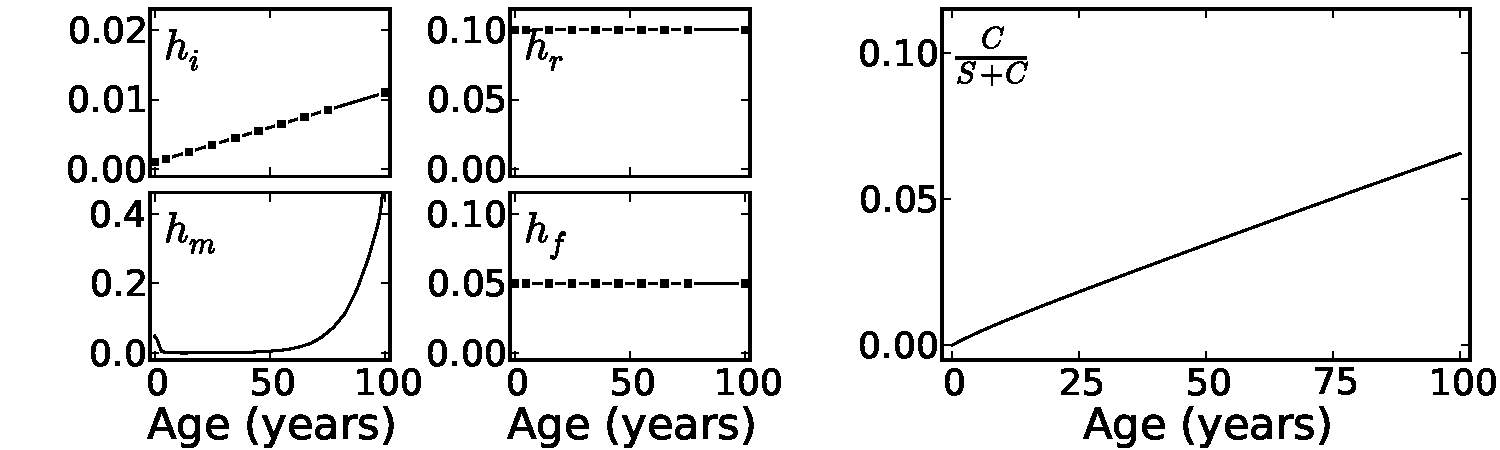
\includegraphics[width=\textwidth]{initial.pdf}
\caption{Consistent disease parameters for a condition where incidence ($i$) increases linearly as a function of age, while remission ($r$) and excess-mortality ($f$) rates are constant. The background mortality ($m$) has an age-specific rate corresponding to females in the sub-Saharan, Southern region in 1990. For a condition with prevalence of zero at age zero, these rates lead to a nearly linear increase as a function of age.}
\label{forward-sim-ex1}
\end{center}
\end{figure}

When I change the age pattern of excess-mortality to also be linearly increasing as a function of age, the consistent prevalence curve becomes more clearly non-linear, showing a condition which gains in prevalence quickly in young age groups, but slower in older ages. Figure~\ref{forward-sim-more-excess-mortality} shows the results of this change.

\begin{figure}[h]
\begin{center}
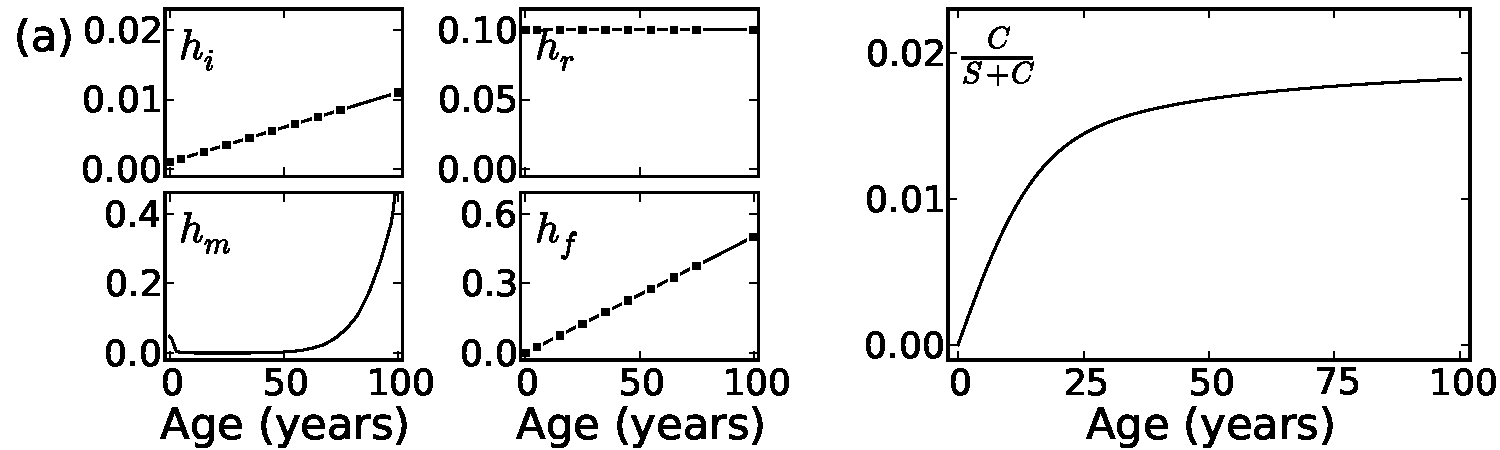
\includegraphics[width=\textwidth]{more-excess-mortality.pdf}

\caption{Consistent disease parameters for a condition where incidence ($i$) and excess-mortality ($f$) both increase linearly as a function of age, while remission ($r$) is constant. The background mortality ($m$) has an age-specific rate corresponding to females in the sub-Saharan Africa, Southern region in 1990. For a condition with prevalence of zero at age zero, these rates drive a prevalence age pattern which increases quickly in young age groups and then more slowly in older age groups.}
\label{forward-sim-more-excess-mortality}
\end{center}
\end{figure}


Although the prevalence age pattern is largely determined by the remission, incidence, and mortality rates, the birth prevalence can also change the shape dramatically.  Here are the results of the same remission, incidence, and mortality rates as in Figure~TK-more-excess-mortality, but with a birth prevalence of 2\%.  Figure~\ref{forward-sim-birth-prevalence} shows how this changes the prevalence after birth.

\begin{figure}[h]
\begin{center}

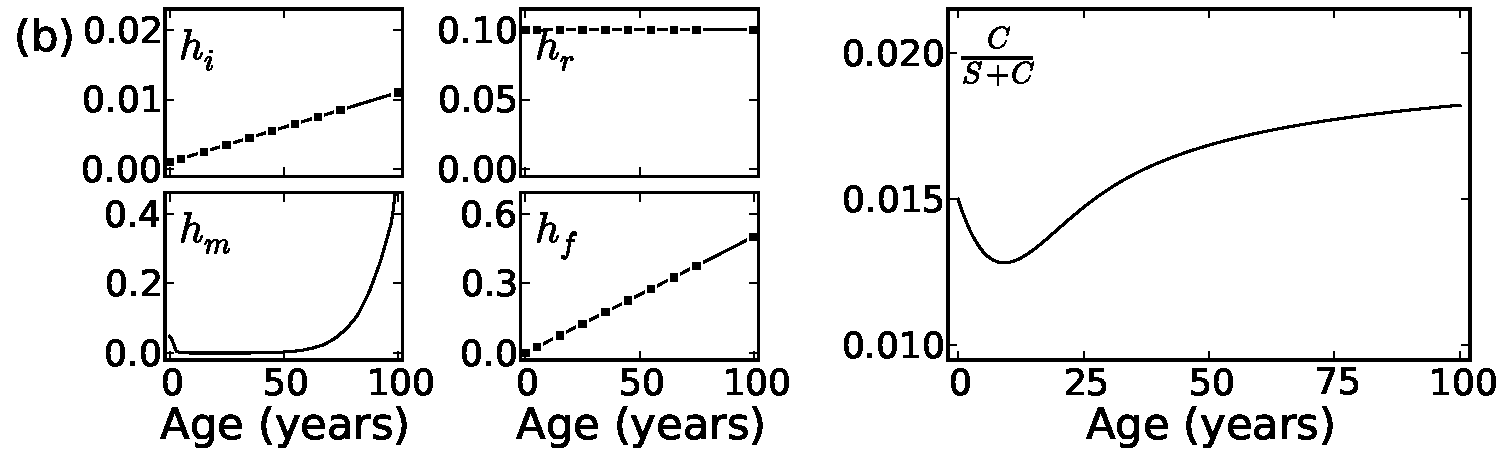
\includegraphics[width=\textwidth]{birth-prevalence.pdf}

\caption{Consistent disease parameters for a condition with non-zero birth prevalence.  The age-specific rates are the same as in Figure~TK-more-excess-mortality: incidence ($i$) and excess-mortality ($f$) both increase linearly as a function of age, while remission ($r$) is constant. The background mortality ($m$) has an age-specific rate corresponding to females in the sub-Saharan Africa, Southern region in 1990. For a condition with prevalence of 2\% at age zero, these rates yield a prevalence age pattern which is highly non-linear, dipping to a minimum of 1.3\% at age 14, and then increasing back up to 1.8\% at oldest ages.}
\label{forward-sim-birth-prevalence}
\end{center}
\end{figure}


To summarize, this series of figures has shown the intuitive and less-than-intuitive way that the levels and age patterns of different epidemiological parameters must be interrelated to satisfy the fundamental equations of population health (when disease rates for each age are changing negligibly slowly as a function of time).

The next series of figures continues to build familiarity with the features of consistent disease modeling, by selecting age patterns for certain rates based on toy models of a variety of diseases.  For example, for a disorder like depression, for which there is primarily incidence in early adulthood, high remission rate, and low excess mortality, the consistency conditions produce a prevalence age pattern that peaks at age 25, as shown in Figure~\ref{forward-sim_mental}.

\begin{figure}
\begin{center}
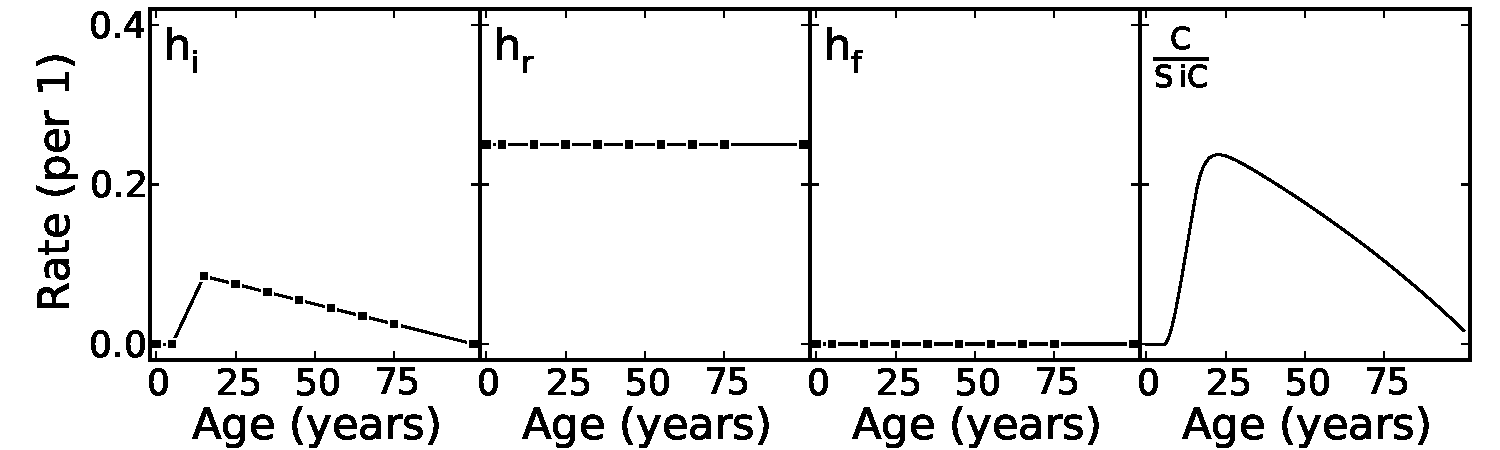
\includegraphics[width=\textwidth]{forward-sim-mental.pdf}
\caption{
In a disorder like depression, the excess-mortality rate is very low, and the remission rate is substantial.  In this case, the age-pattern of the incidence rate drives the age pattern of prevalence in a slightly non-linear fashion, where the age pattern of prevalence is a ``smoothed'' copy the incidence age pattern.
}
\label{forward-sim_mental}
\end{center}
\end{figure}

For a congenital disorder, like Down's Syndrome, with birth prevalence, no incidence after birth, no remission, and substantial mortality, the consistent prevalence age pattern is shown in Figure~\ref{forward-sim-congenital}.

\begin{figure}[h]
\begin{center}
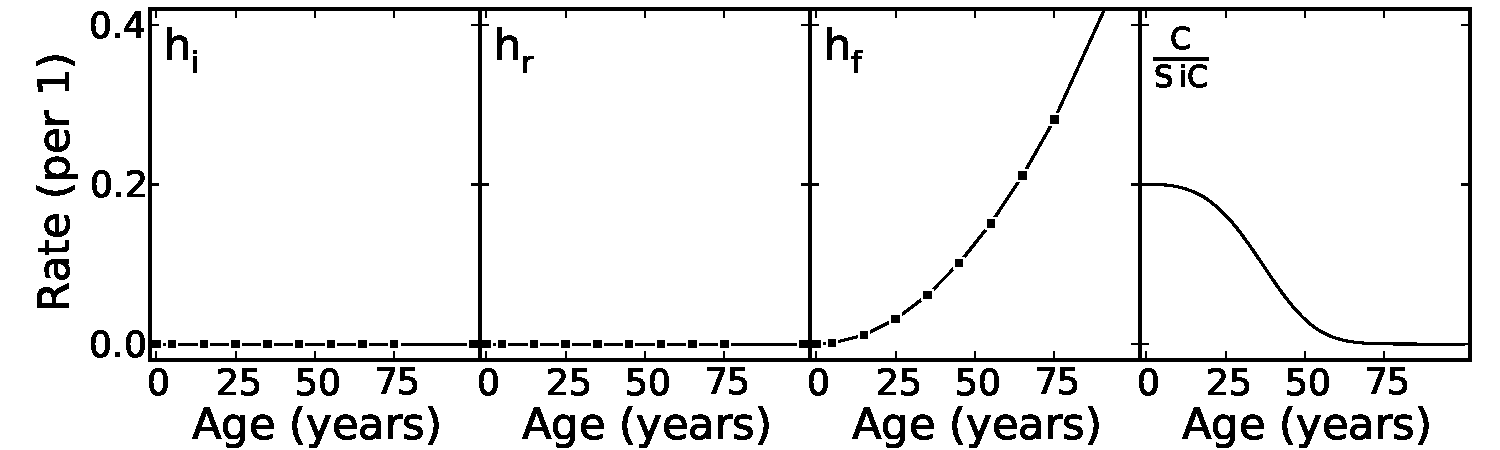
\includegraphics[width=\textwidth]{forward-sim-congenital.pdf}
\caption{For a condition acquired before or during birth, such as Down's Syndrome, incidence and remission are often very low, while excess-mortality may increase with age.  This leads to prevalence that decreases as a function of age.}
\label{forward-sim-congenital}
\end{center}
\end{figure}

For a disorder that affects the elderly, like Parkinson's Disease, the consistent age patterns for mortality, incidence, remission, and prevalence could look roughly like the age-specific rates shown in Figure~\ref{forward-sim-old-age}.

\begin{figure}[h]
\begin{center}
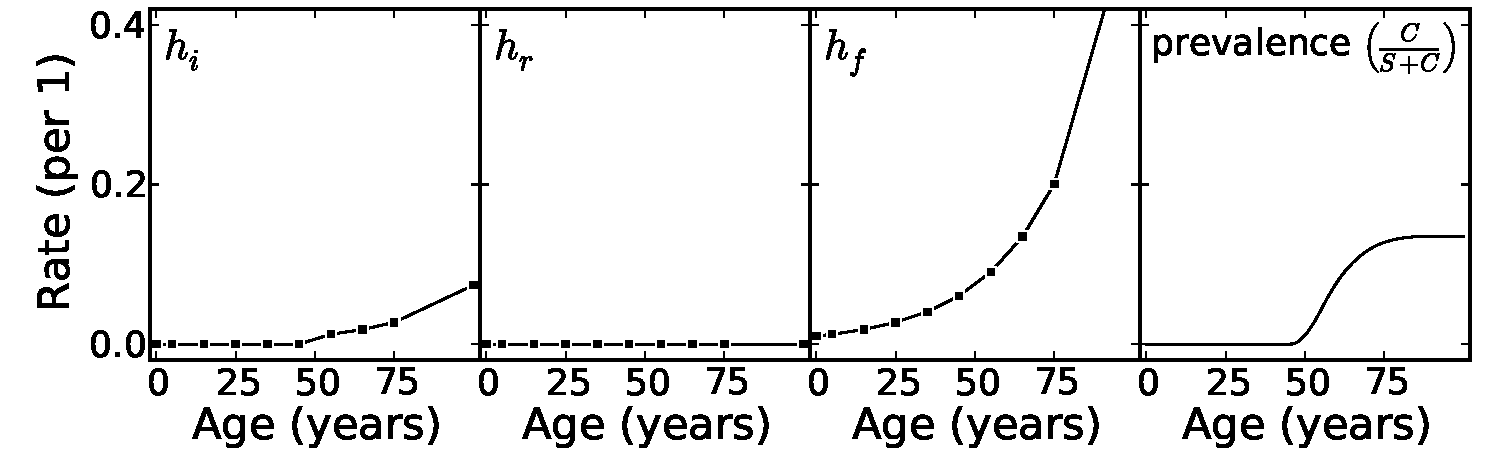
\includegraphics[width=\textwidth]{forward-sim-old_age.pdf}
\caption{For a condition that occurs in older age groups, such as Parkinson's Disease, the age-specific rates may look like these, where increasing incidence drives increasing prevalence in older age groups, but the countervailing force of increasing excess-mortality causes the prevalence increase to level out, or even decline at oldest ages.}
\label{forward-sim-old-age}
\end{center}
\end{figure}

And for disorders related to reproductive health, like premenstrual syndrome, with zero excess mortality, incidence during ages 15-60, and remission that increases substantially at age 55, the consistent age patterns could look like those shown in Figure~\ref{forward-sim-reproductive}.

\begin{figure}[h]
\begin{center}
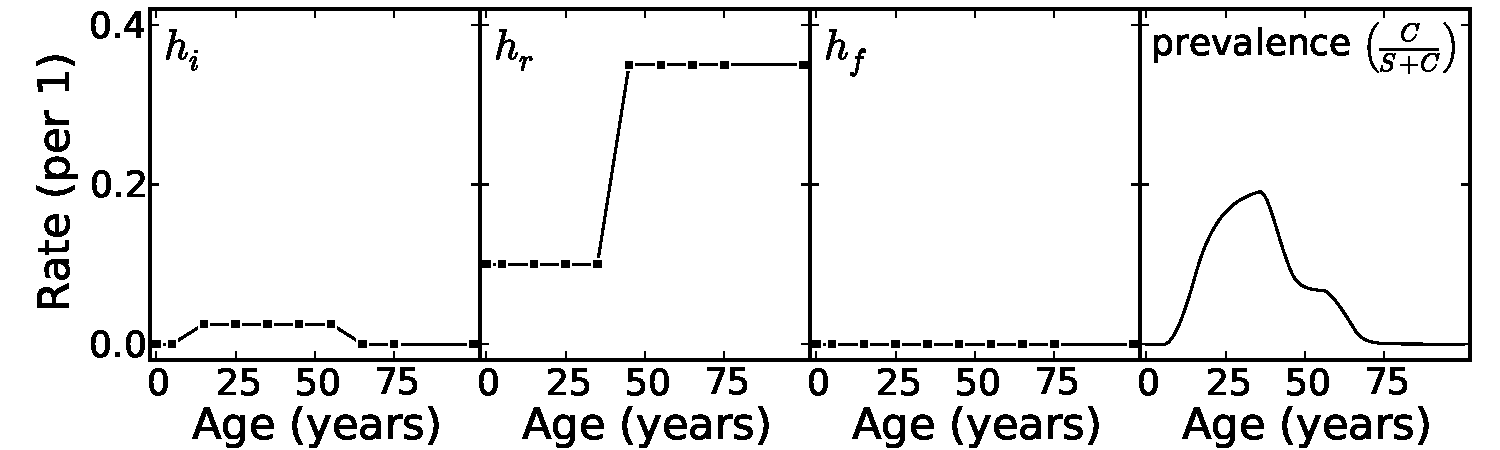
\includegraphics[width=\textwidth]{forward-sim-reproductive.pdf}
\caption{For a condition related to reproductive health, like premenstrual syndrome, the age-specific rates may look like these, where incidence is non-zero during reproductive ages, and zero in the very young and old, and remission increases steeply at age 50. This age pattern, with some shifts in age groups is also similar to that seen in data on substance dependence.}
\label{forward-sim-reproductive}
\end{center}
\end{figure}



To conclude this series of plots, I've included an ``incidence impulse response'' example, showing the prevalence produced to be consistent with an incidence pattern that is only non-zero for a single age group. This is the content of Figure~\ref{forward-sim-incidence-pluse}.

\begin{figure}[h]
\begin{center}

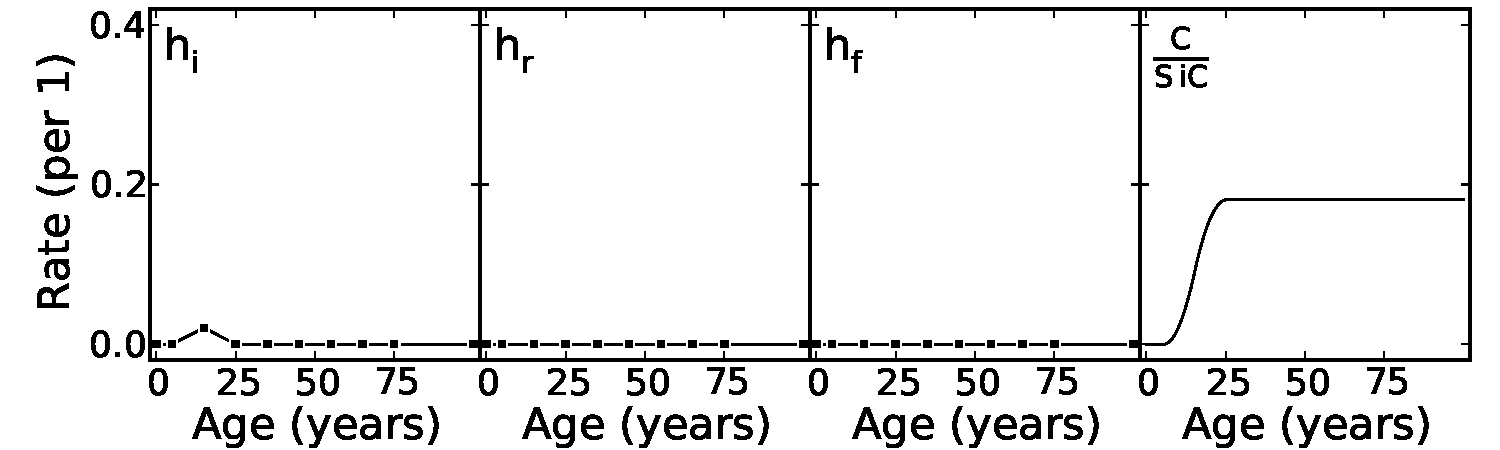
\includegraphics[width=\textwidth]{forward-sim-incidence_pulse.pdf}

\caption{The results of an ``incidence pulse'' show how the system responds to a condition with no excess-mortality and no remission that is incident only for a limited number of young ages.  This incidence age function produces a sigmoidal age pattern in prevalence, which transitions from zero to non-zero during the ages that incidence is non-zero, and then stays at this value for all older ages.}
\label{forward-sim-incidence-pluse}
\end{center}
\end{figure}



Forward simulations such as these are the foundation of my approach to validate model implementations and also to investigate the performance of the model when model assumptions are violated. The details of this sort of simulation study is a topic that I will return to in Section~\ref{TK}.

TK The simulation study approach can be described in full detail here as well, and can serve as justification for decisions described in the next two chapters.

\subsection{What happens to prevalence when the disease incidence or remission or mortality is not constant over time?}

Certain important diseases such as diabetes are widely believed to have substantial changes in incidence, remission, and mortality rates over time.  What is the effect of the endemic equilibrium assumption of the age-specific prevalence? TK plots comparing prevalence from a synthetic cohort model to a period model using simulation data.

\subsection{Computational aspects of forward simulation}
There are several computational optimizations of the forward simulation that are discussed in this section.  Because the statistical inference technique will require simulating the compartmental model for thousands or millions of different parameter settings, speed is of the essence.
TK discussion of different approaches to solving the differential equations: exact solution, numerical solution. Stiff versus non-stiff numerical solution. Approximation when remission rate is very high.
